\documentclass{article}\usepackage[]{graphicx}\usepackage[]{color}
%% maxwidth is the original width if it is less than linewidth
%% otherwise use linewidth (to make sure the graphics do not exceed the margin)
\makeatletter
\def\maxwidth{ %
  \ifdim\Gin@nat@width>\linewidth
    \linewidth
  \else
    \Gin@nat@width
  \fi
}
\makeatother

\definecolor{fgcolor}{rgb}{0.345, 0.345, 0.345}
\newcommand{\hlnum}[1]{\textcolor[rgb]{0.686,0.059,0.569}{#1}}%
\newcommand{\hlstr}[1]{\textcolor[rgb]{0.192,0.494,0.8}{#1}}%
\newcommand{\hlcom}[1]{\textcolor[rgb]{0.678,0.584,0.686}{\textit{#1}}}%
\newcommand{\hlopt}[1]{\textcolor[rgb]{0,0,0}{#1}}%
\newcommand{\hlstd}[1]{\textcolor[rgb]{0.345,0.345,0.345}{#1}}%
\newcommand{\hlkwa}[1]{\textcolor[rgb]{0.161,0.373,0.58}{\textbf{#1}}}%
\newcommand{\hlkwb}[1]{\textcolor[rgb]{0.69,0.353,0.396}{#1}}%
\newcommand{\hlkwc}[1]{\textcolor[rgb]{0.333,0.667,0.333}{#1}}%
\newcommand{\hlkwd}[1]{\textcolor[rgb]{0.737,0.353,0.396}{\textbf{#1}}}%

\usepackage{framed}
\makeatletter
\newenvironment{kframe}{%
 \def\at@end@of@kframe{}%
 \ifinner\ifhmode%
  \def\at@end@of@kframe{\end{minipage}}%
  \begin{minipage}{\columnwidth}%
 \fi\fi%
 \def\FrameCommand##1{\hskip\@totalleftmargin \hskip-\fboxsep
 \colorbox{shadecolor}{##1}\hskip-\fboxsep
     % There is no \\@totalrightmargin, so:
     \hskip-\linewidth \hskip-\@totalleftmargin \hskip\columnwidth}%
 \MakeFramed {\advance\hsize-\width
   \@totalleftmargin\z@ \linewidth\hsize
   \@setminipage}}%
 {\par\unskip\endMakeFramed%
 \at@end@of@kframe}
\makeatother

\definecolor{shadecolor}{rgb}{.97, .97, .97}
\definecolor{messagecolor}{rgb}{0, 0, 0}
\definecolor{warningcolor}{rgb}{1, 0, 1}
\definecolor{errorcolor}{rgb}{1, 0, 0}
\newenvironment{knitrout}{}{} % an empty environment to be redefined in TeX

\usepackage{alltt}
\usepackage[sc]{mathpazo}
\usepackage[T1]{fontenc}
\usepackage{geometry}
\geometry{verbose,tmargin=2.5cm,bmargin=2.5cm,lmargin=2.5cm,rmargin=2.5cm}
\setcounter{secnumdepth}{2}
\setcounter{tocdepth}{2}
\usepackage{url}
\usepackage[unicode=true,pdfusetitle,
 bookmarks=true,bookmarksnumbered=true,bookmarksopen=true,bookmarksopenlevel=2,
 breaklinks=false,pdfborder={0 0 1},backref=false,colorlinks=false]
 {hyperref}
\hypersetup{
 pdfstartview={XYZ null null 1}}
\usepackage{breakurl}
\IfFileExists{upquote.sty}{\usepackage{upquote}}{}
\begin{document}




\author{Ricky Lim}
\title{David \& Goliath: Sentiment Analysis}
\maketitle

\begin{verbatim}
  Filename: sentimentPlot.Rnw 
  Working directory: /Users/RickyLim/Dropbox/RandomWalk/DavidGoliath/Ranalysis 
\end{verbatim}

\section{Background}
The background of this analysis was described \href{https://github.com/rickylim19/DavidGoliath}{here}


\section{Content}
\subsection{Data Loaded}
\begin{knitrout}
\definecolor{shadecolor}{rgb}{0.969, 0.969, 0.969}\color{fgcolor}\begin{kframe}
\begin{alltt}
\hlcom{# from different bible versions}
\hlstd{ESV_sentiment} \hlkwb{<-} \hlkwd{read.delim}\hlstd{(}\hlstr{"../data/ESV_sentimentAnalysis.txt"}\hlstd{,} \hlkwc{header} \hlstd{=} \hlnum{FALSE}\hlstd{)}
\hlstd{KJV_sentiment} \hlkwb{<-} \hlkwd{read.delim}\hlstd{(}\hlstr{"../data/KJV_sentimentAnalysis.txt"}\hlstd{,} \hlkwc{header} \hlstd{=} \hlnum{FALSE}\hlstd{)}
\hlstd{NIV_sentiment} \hlkwb{<-} \hlkwd{read.delim}\hlstd{(}\hlstr{"../data/NIV_sentimentAnalysis.txt"}\hlstd{,} \hlkwc{header} \hlstd{=} \hlnum{FALSE}\hlstd{)}
\end{alltt}
\end{kframe}
\end{knitrout}


\subsection{Plot Constructed}
\begin{kframe}
\begin{alltt}
\hlcom{# construct plot for sentiment probabilities from these three versions}
\hlkwd{library}\hlstd{(ggplot2)}
\hlstd{p} \hlkwb{<-} \hlkwd{ggplot}\hlstd{(ESV_sentiment,} \hlkwd{aes}\hlstd{(}\hlkwc{x}\hlstd{=V1,} \hlkwc{y}\hlstd{=V2))}\hlopt{+}
     \hlkwd{stat_smooth}\hlstd{(}\hlkwd{aes}\hlstd{(}\hlkwc{color}\hlstd{=}\hlstr{"ESV"}\hlstd{))}\hlopt{+}
     \hlkwd{stat_smooth}\hlstd{(}\hlkwc{data}\hlstd{=KJV_sentiment,} \hlkwd{aes}\hlstd{(}\hlkwc{color}\hlstd{=}\hlstr{"KJV"}\hlstd{))}\hlopt{+}
     \hlkwd{stat_smooth}\hlstd{(}\hlkwc{data}\hlstd{=NIV_sentiment,} \hlkwd{aes}\hlstd{(}\hlkwc{color}\hlstd{=}\hlstr{"NIV"}\hlstd{))}\hlopt{+}
     \hlkwd{labs}\hlstd{(}\hlkwc{color}\hlstd{=}\hlstr{"Biblical Versions"}\hlstd{)} \hlopt{+}
     \hlkwd{xlab}\hlstd{(}\hlstr{'Biblical Verses'}\hlstd{)} \hlopt{+}
     \hlkwd{ylab}\hlstd{(}\hlstr{'Probability'}\hlstd{)} \hlopt{+}
     \hlkwd{opts}\hlstd{(}\hlkwc{title}\hlstd{=}\hlstr{'Sentiment on David and Goliath'}\hlstd{)}
\hlkwd{ggsave}\hlstd{(}\hlkwc{filename}\hlstd{=}\hlstr{'../img/sentimentPlot.png'}\hlstd{,} \hlkwc{plot} \hlstd{= p)}
\end{alltt}
\end{kframe}


\begin{knitrout}
\definecolor{shadecolor}{rgb}{0.969, 0.969, 0.969}\color{fgcolor}\begin{kframe}
\begin{alltt}
\hlcom{# insert saved figure from above}
\hlkwd{library}\hlstd{(knitr)}
\hlstd{f} \hlkwb{<-} \hlstr{"../img/sentimentPlot"}
\end{alltt}
\end{kframe}
\end{knitrout}

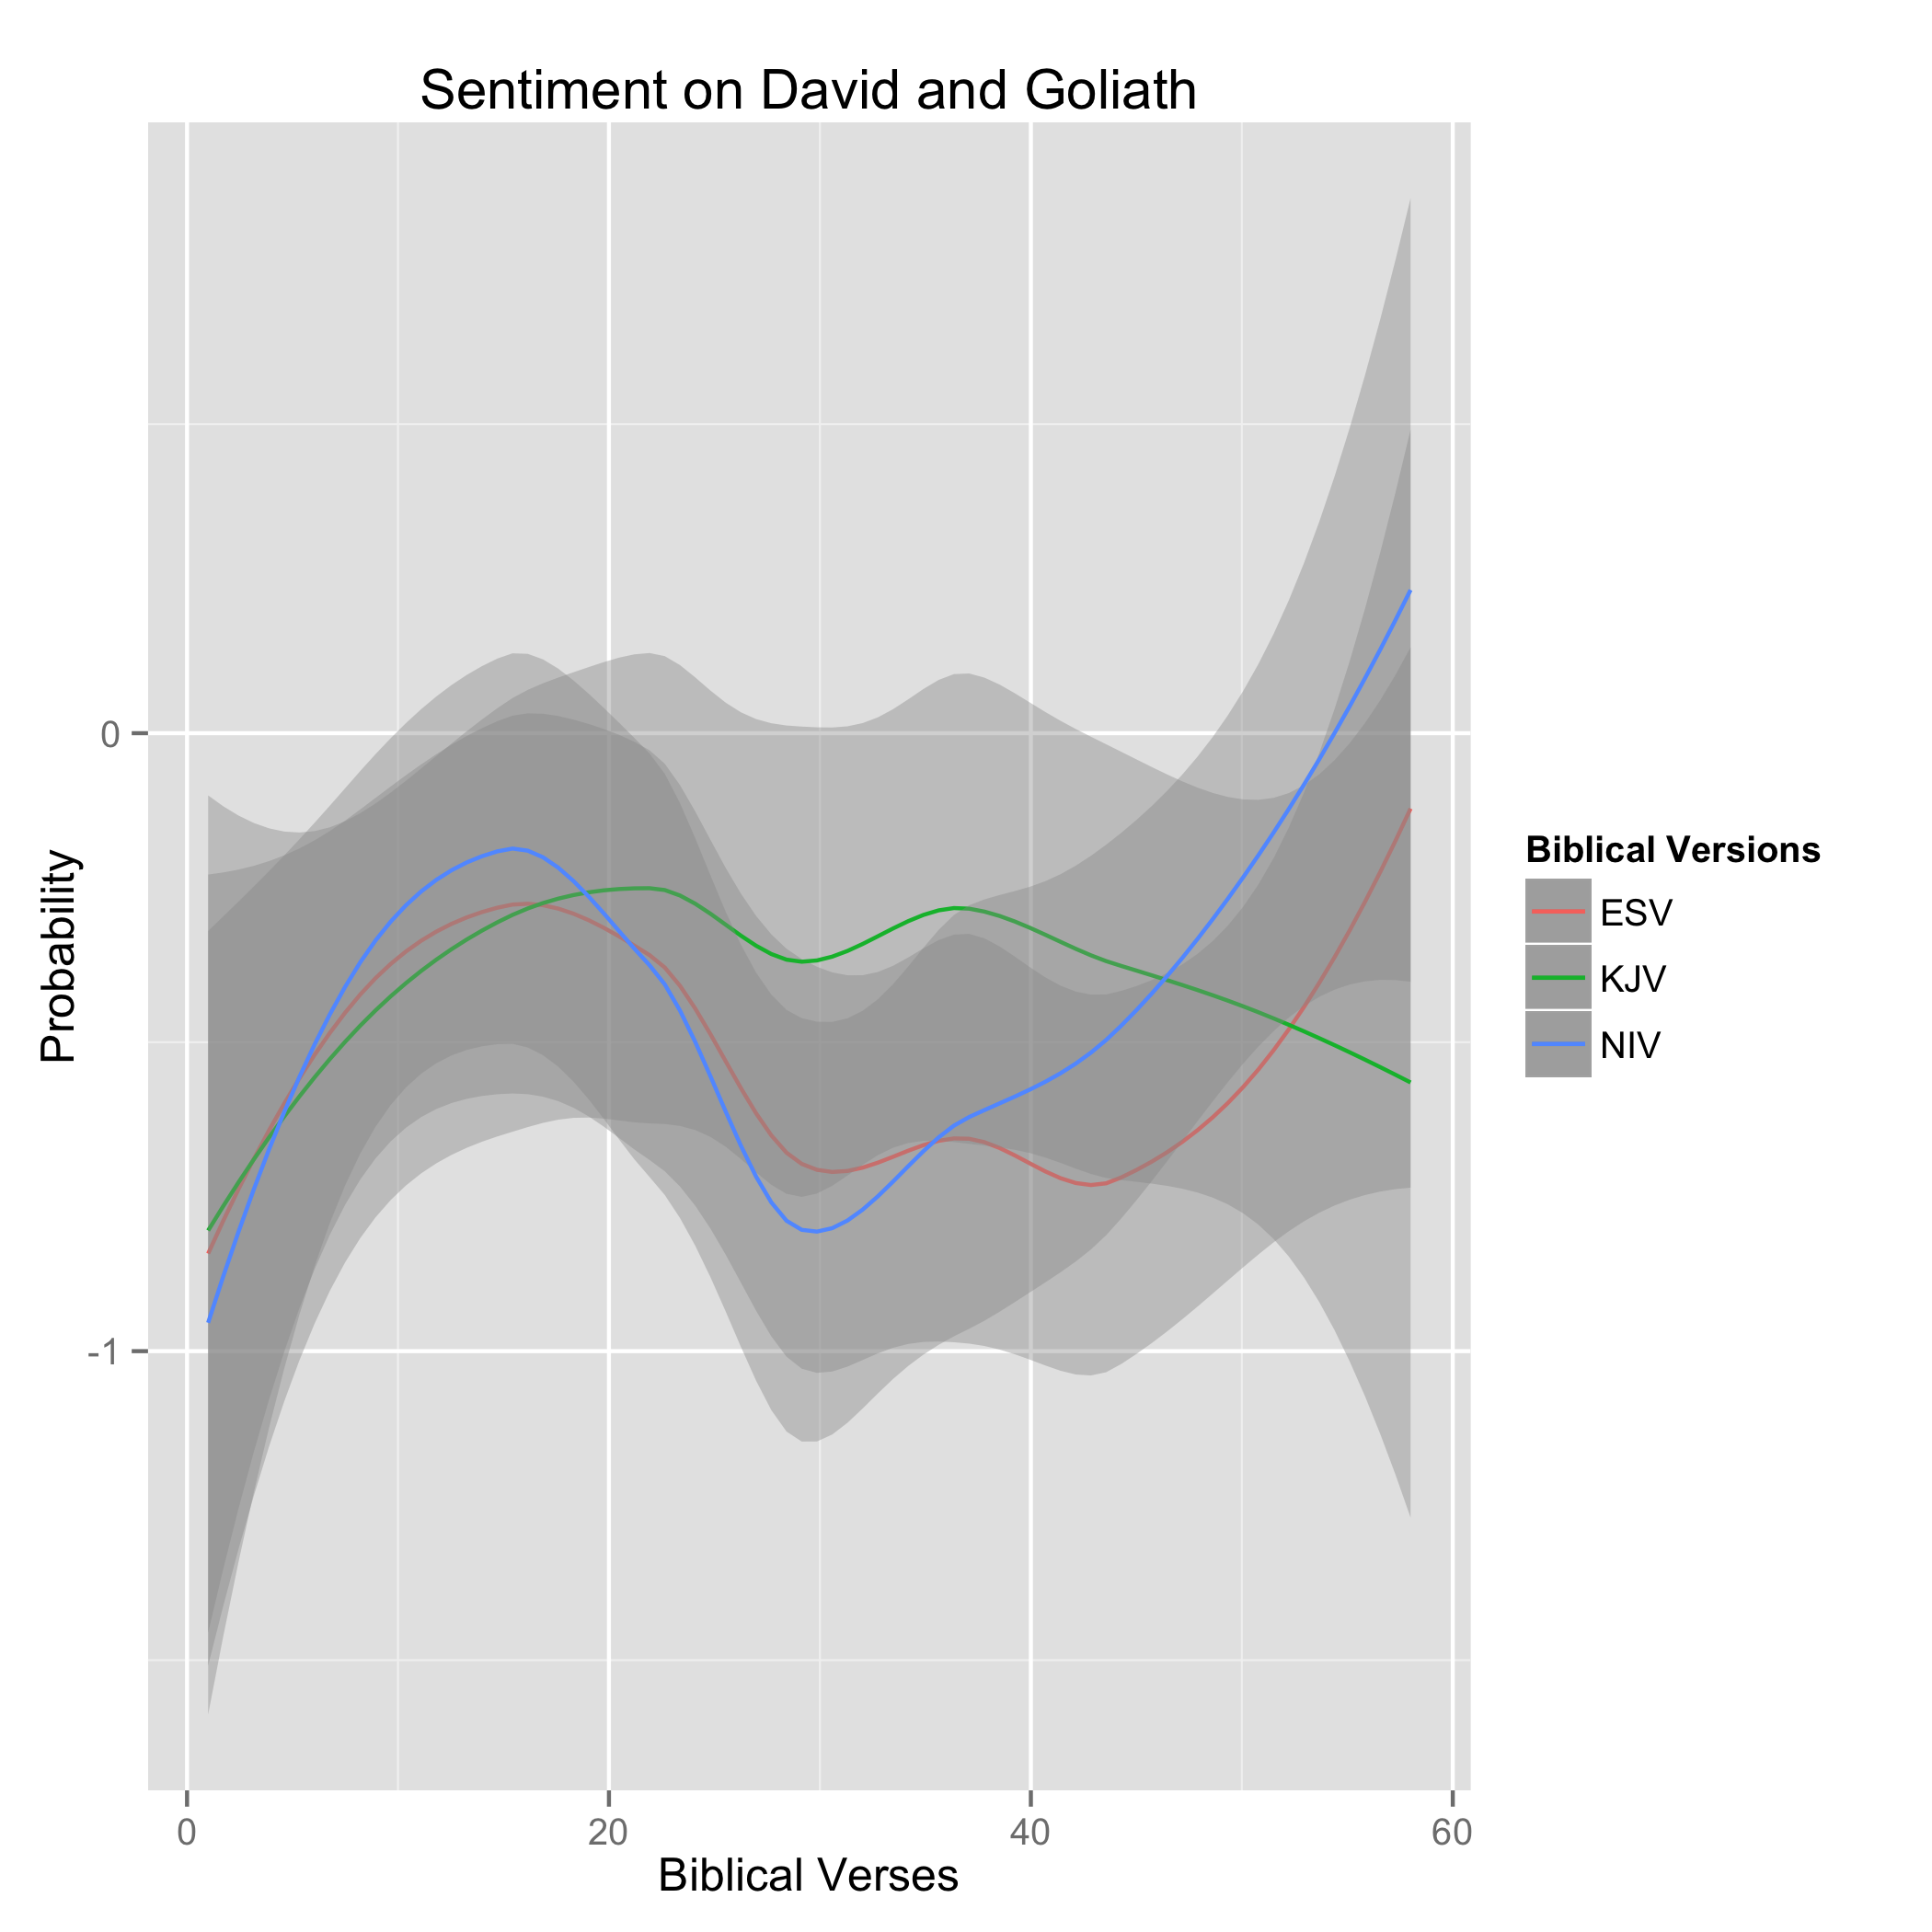
\includegraphics[width=500px,height=300px]{../img/sentimentPlot}

\subsection{Correlation Checked}
\begin{kframe}
\begin{alltt}
\hlcom{# merge three biblical versions based on their verses}
\hlstd{ESV_KJV} \hlkwb{<-} \hlkwd{merge}\hlstd{(ESV_sentiment, KJV_sentiment,} \hlkwc{by.x} \hlstd{=} \hlstr{"V1"}\hlstd{,} \hlkwc{by.y} \hlstd{=} \hlstr{"V1"}\hlstd{)}
\hlstd{ESV_KJV_NIV} \hlkwb{<-} \hlkwd{merge}\hlstd{(ESV_KJV, NIV_sentiment,} \hlkwc{by.x} \hlstd{=} \hlstr{"V1"}\hlstd{,} \hlkwc{by.y} \hlstd{=} \hlstr{"V1"}\hlstd{)}

\hlcom{# label this dataframe}
\hlkwd{colnames}\hlstd{(ESV_KJV_NIV)} \hlkwb{<-} \hlkwd{c}\hlstd{(}\hlstr{"Verse"}\hlstd{,} \hlstr{"ESV"}\hlstd{,} \hlstr{"KJV"}\hlstd{,} \hlstr{"NIV"}\hlstd{)}
\hlkwd{rownames}\hlstd{(ESV_KJV_NIV)} \hlkwb{<-} \hlstd{ESV_KJV_NIV[,} \hlnum{1}\hlstd{]}
\hlstd{ESV_KJV_NIV} \hlkwb{<-} \hlstd{ESV_KJV_NIV[,} \hlnum{2}\hlopt{:}\hlnum{4}\hlstd{]}

\hlcom{# compute the correlation using spearman}
\hlstd{cor_tab} \hlkwb{<-} \hlkwd{cor}\hlstd{(ESV_KJV_NIV,} \hlkwc{method} \hlstd{=} \hlstr{"spearman"}\hlstd{)}

\hlcom{# create table for latex}
\hlkwd{library}\hlstd{(xtable)}
\hlkwd{print}\hlstd{(}\hlkwd{xtable}\hlstd{(cor_tab,} \hlkwc{caption} \hlstd{=} \hlstr{"Correlation among Three Versions"}\hlstd{))}
\end{alltt}
\end{kframe}% latex table generated in R 3.0.2 by xtable 1.7-1 package
% Wed Nov 13 14:33:03 2013
\begin{table}[ht]
\centering
\begin{tabular}{rrrr}
  \hline
 & ESV & KJV & NIV \\ 
  \hline
ESV & 1.00 & 0.58 & 0.69 \\ 
  KJV & 0.58 & 1.00 & 0.24 \\ 
  NIV & 0.69 & 0.24 & 1.00 \\ 
   \hline
\end{tabular}
\caption{Correlation among Three Versions} 
\end{table}




\subsection{Overall Sentiment}
\begin{kframe}
\begin{alltt}
\hlkwd{print}\hlstd{(}\hlkwd{xtable}\hlstd{(}\hlkwd{summary}\hlstd{(ESV_KJV_NIV),} \hlkwc{caption} \hlstd{=} \hlstr{"Stat Overview"}\hlstd{))}
\end{alltt}
\end{kframe}% latex table generated in R 3.0.2 by xtable 1.7-1 package
% Wed Nov 13 14:56:41 2013
\begin{table}[ht]
\centering
\begin{tabular}{rlll}
  \hline
 &      ESV &      KJV &      NIV \\ 
  \hline
1 & Min.   :-1.000   & Min.   :-0.999   & Min.   :-0.999   \\ 
  2 & 1st Qu.:-0.923   & 1st Qu.:-0.922   & 1st Qu.:-0.911   \\ 
  3 & Median :-0.804   & Median :-0.761   & Median :-0.725   \\ 
  4 & Mean   :-0.527   & Mean   :-0.397   & Mean   :-0.413   \\ 
  5 & 3rd Qu.:-0.603   & 3rd Qu.: 0.572   & 3rd Qu.: 0.244   \\ 
  6 & Max.   : 0.991   & Max.   : 0.973   & Max.   : 0.988   \\ 
   \hline
\end{tabular}
\caption{Stat Overview} 
\end{table}
\begin{kframe}\begin{alltt}
\hlstd{MostPositive} \hlkwb{<-} \hlkwd{apply}\hlstd{(ESV_KJV_NIV,} \hlnum{2}\hlstd{, which.max)}
\hlstd{MostNegative} \hlkwb{<-} \hlkwd{apply}\hlstd{(ESV_KJV_NIV,} \hlnum{2}\hlstd{, which.min)}
\hlstd{MostSentiment} \hlkwb{<-} \hlkwd{cbind}\hlstd{(MostPositive, MostNegative)}
\hlkwd{print}\hlstd{(}\hlkwd{xtable}\hlstd{(MostSentiment,} \hlkwc{caption} \hlstd{=} \hlstr{"Most Sentimented Verses"}\hlstd{))}
\end{alltt}
\end{kframe}% latex table generated in R 3.0.2 by xtable 1.7-1 package
% Wed Nov 13 14:56:41 2013
\begin{table}[ht]
\centering
\begin{tabular}{rrr}
  \hline
 & MostPositive & MostNegative \\ 
  \hline
ESV &  18 &  51 \\ 
  KJV &  38 &   8 \\ 
  NIV &  18 &   7 \\ 
   \hline
\end{tabular}
\caption{Most Sentimented Verses} 
\end{table}



\section{Metainfo}
\begin{knitrout}
\definecolor{shadecolor}{rgb}{0.969, 0.969, 0.969}\color{fgcolor}\begin{kframe}
\begin{alltt}
\hlkwd{sessionInfo}\hlstd{()}
\end{alltt}
\begin{verbatim}
## R version 3.0.2 (2013-09-25)
## Platform: x86_64-apple-darwin11.4.2 (64-bit)
## 
## locale:
## [1] en_US.UTF-8/en_US.UTF-8/en_US.UTF-8/C/en_US.UTF-8/en_US.UTF-8
## 
## attached base packages:
## [1] stats     graphics  grDevices utils     datasets  methods   base     
## 
## other attached packages:
## [1] reshape2_1.2.2  codetools_0.2-8 knitr_1.5       xtable_1.7-1    ggplot2_0.9.3.1
## 
## loaded via a namespace (and not attached):
##  [1] Cairo_1.5-2        colorspace_1.2-4   dichromat_2.0-0    digest_0.6.3      
##  [5] evaluate_0.5.1     formatR_0.10       grid_3.0.2         gtable_0.1.2      
##  [9] highr_0.3          labeling_0.2       MASS_7.3-29        munsell_0.4.2     
## [13] plyr_1.8           proto_0.3-10       RColorBrewer_1.0-5 scales_0.2.3      
## [17] stringr_0.6.2      tools_3.0.2
\end{verbatim}
\end{kframe}
\end{knitrout}


\begin{knitrout}
\definecolor{shadecolor}{rgb}{0.969, 0.969, 0.969}\color{fgcolor}\begin{kframe}
\begin{alltt}
\hlkwd{library}\hlstd{(knitr)}
\hlkwd{knit}\hlstd{(}\hlstr{"sentimentPlot.Rnw"}\hlstd{)}  \hlcom{# compile to tex}
\end{alltt}


{\ttfamily\noindent\bfseries\color{errorcolor}{\#\# Error: duplicate label 'setup'}}\begin{alltt}
\hlkwd{purl}\hlstd{(}\hlstr{"sentimentPlot.Rnw"}\hlstd{,} \hlkwc{documentation} \hlstd{=} \hlnum{0}\hlstd{)}  \hlcom{# extract R code only}
\hlkwd{knit2pdf}\hlstd{(}\hlstr{"sentimentPlot.Rnw"}\hlstd{)}
\end{alltt}


{\ttfamily\noindent\bfseries\color{errorcolor}{\#\# Error: duplicate label 'setup'}}\end{kframe}
\end{knitrout}


\end{document}

